\section{Validation results and uncertainty}
\label{app:validation}

% Validation tables moved from the report; the main text uses the test set.

\resulttable{stage1_pretrained_accuracy}
\resulttable{stage1_scratch_accuracy}
\resulttable{stage1_pretrained_accuracy_sd_prompt}
\resulttable{stage1_pretrained_accuracy_vs_randaugment}
\resulttable{stage1_scratch_accuracy_vs_randaugment}

\section{Seed intervals and image bootstrap}
\label{app:bootstrap}
% Moved from the report's error analysis (validation predictions; no retraining, test set unused).
\todo{move the report's uncertainty paragraph here, updated to five seeds}

\resulttable{stage1_pretrained_bootstrap}
\resulttable{stage1_scratch_bootstrap}

\section{Per-superclass changes}
\label{app:superclass}

\begin{figure}[H]
	\centering
	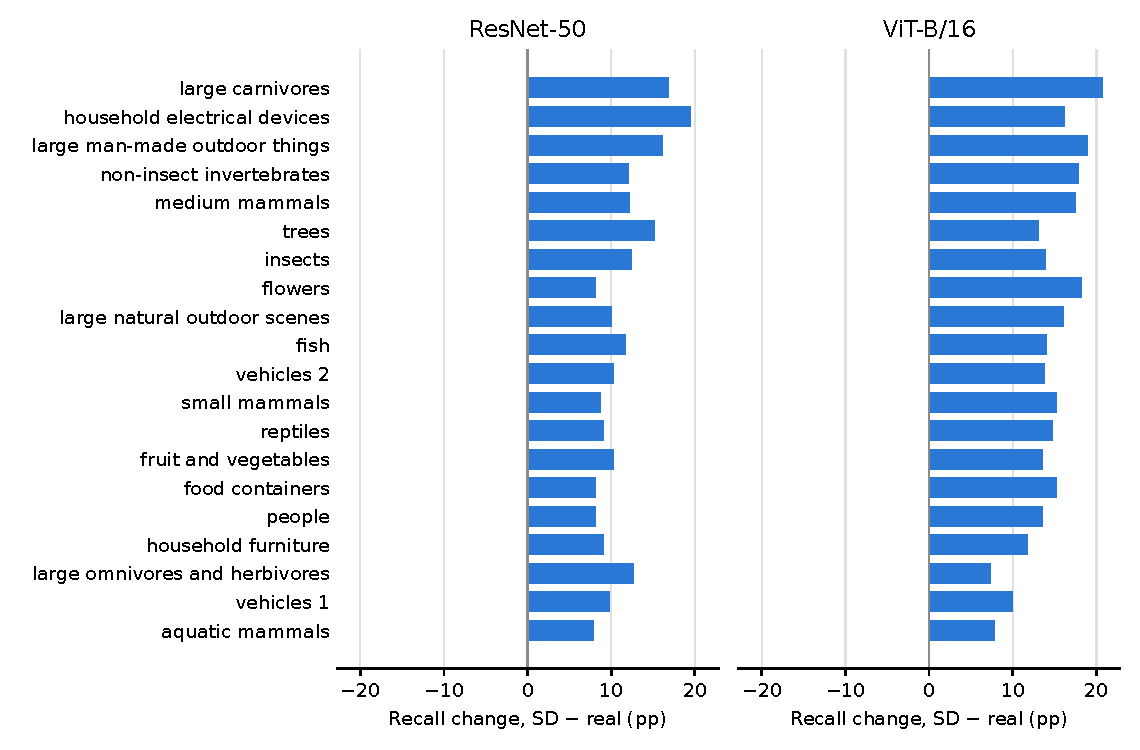
\includegraphics[width=0.85\textwidth]{stage1_pretrained_b5_sd_prompt_vs_real_only_superclasses.pdf}
	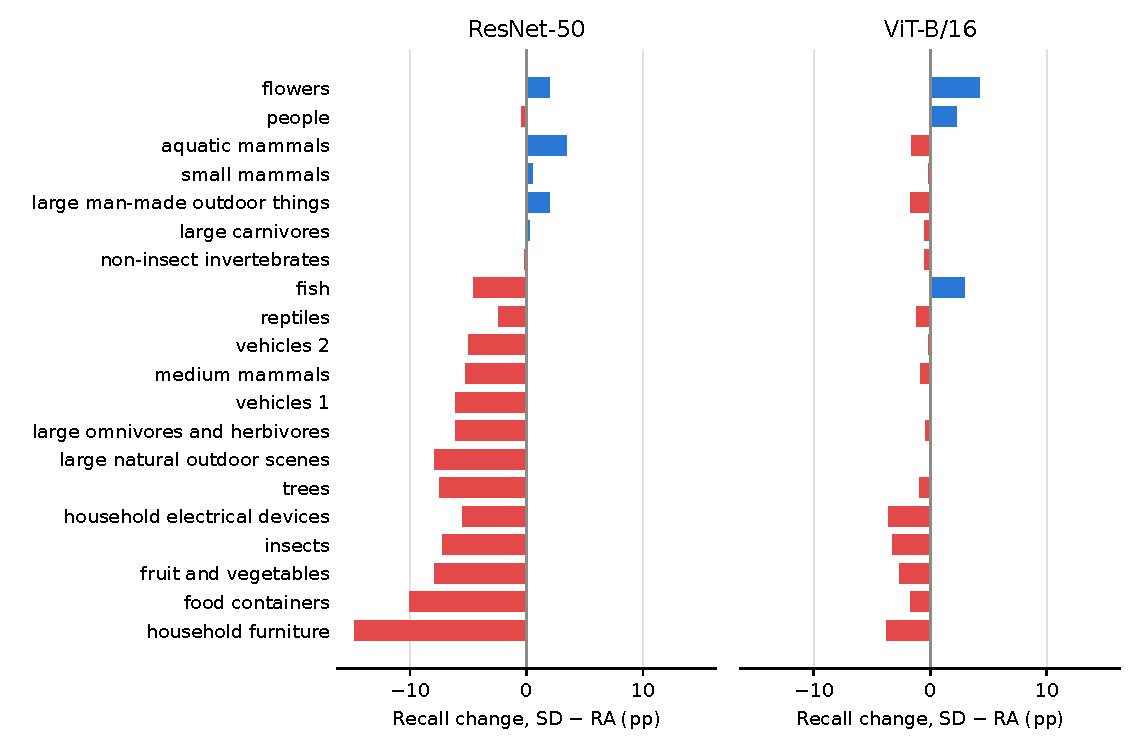
\includegraphics[width=0.85\textwidth]{stage1_scratch_b5_sd_prompt_vs_randaugment_superclasses.pdf}
	\caption{Recall change per CIFAR-100 superclass at 5 images per class, mean over seeds 0 to 4 (top) and 0 to 2 (bottom), in percentage points. Top: class-prompt images minus real-only, ImageNet-pretrained classifiers. Bottom: class-prompt images minus RandAugment, randomly initialized classifiers. Superclasses are sorted by the mean change over both models; blue bars are gains and red bars losses.}
	\label{fig:stage1-superclass}
\end{figure}

\section{Generated samples}
\label{app:samples}

\begin{figure}[H]
	\centering
	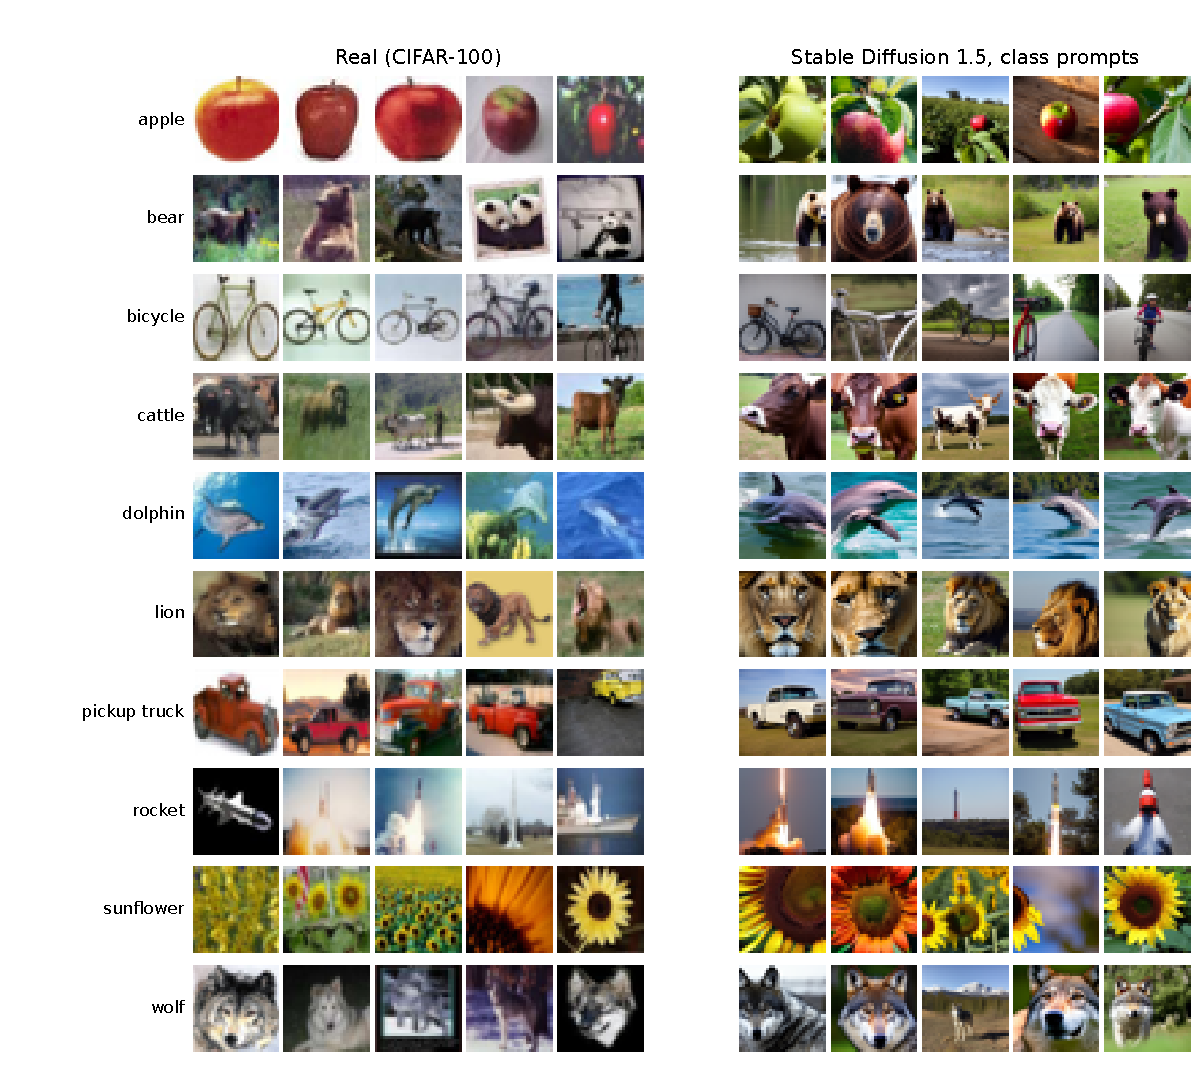
\includegraphics[width=0.8\textwidth]{sd15_prompt_samples.pdf}
	\caption{Samples of the class-prompt pool (pretrained Stable Diffusion 1.5, 32$\times$32 as used for training).}
	\label{fig:sd-samples}
\end{figure}
% TODO: LoRA, img2img and GAN samples side by side.
